\subsection{Overview}
The basic architecture for the system is a Client-Server setup. The server will handle persistent data and contain a small subsystem for manipulating data, we will for now not describe the server or the communication between the server and client greater detail and instead focus on the client.\\

The Client-system will be made with a Model-View-Controller (MVC) architecture. The system should have different views (Log in, MonthView... etc.) which would require different event-handling. The MVC allows this because it makes it easy to do runtime changes of views and controllers. It also results in high cohesion, in that the control objects and the view objects are separated in accordance to their respective responsibilities. Both view and control objects can be separated into small classes that only handles smaller tasks. However creating the MVC-architecture requires extra code. The main architecture can be seen below (it is possible to zoom in), we have not included all views and control objects to keep things a bit clean.

\paragraph{Architecture}
\begin{center}
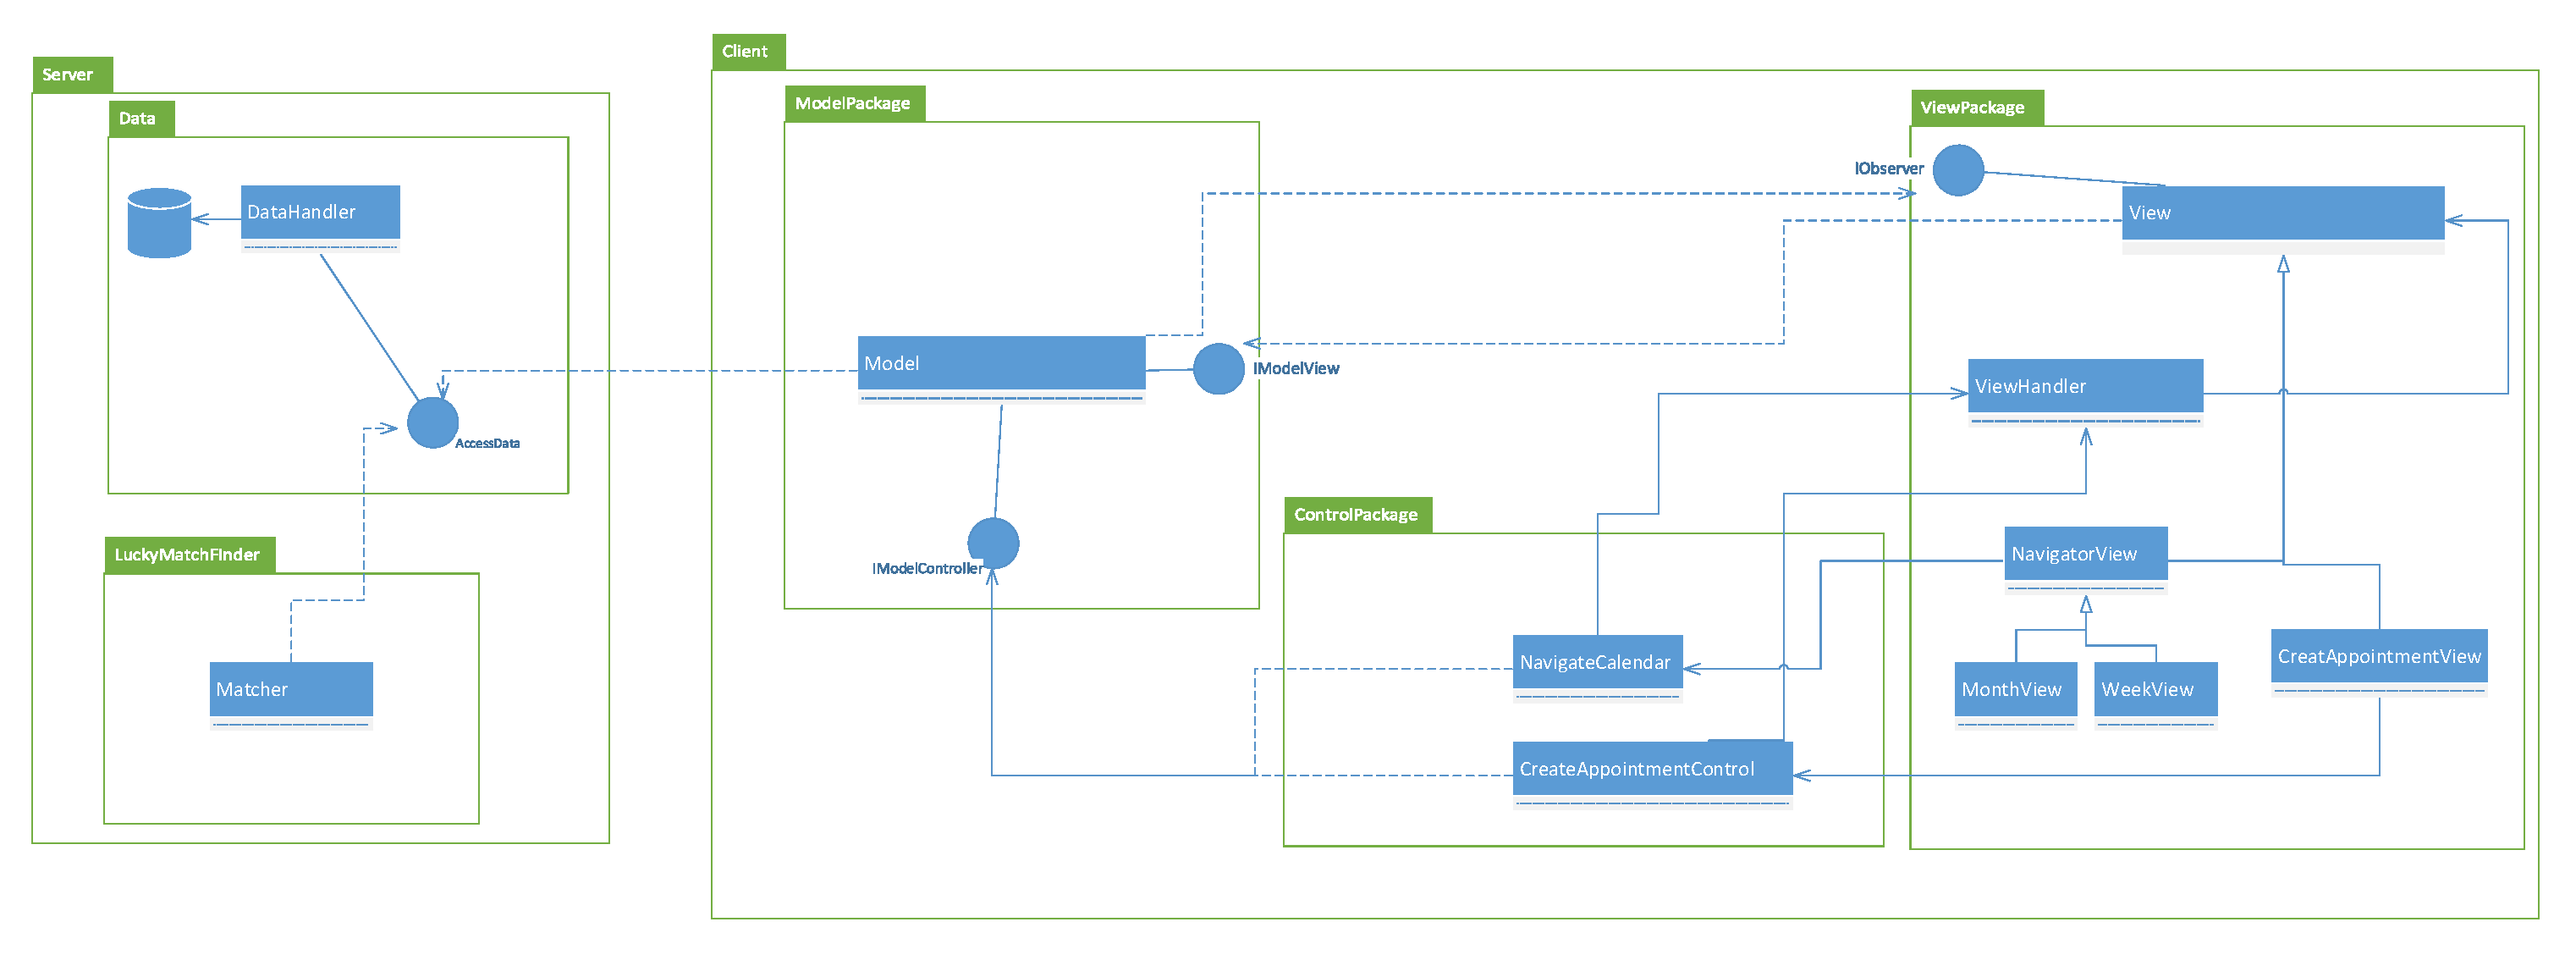
\includegraphics[scale=.4]{sections/Architecture.pdf}
\end{center}
\pagebreak

\subsection{Subsystem decomposition}
The MVC architecture gives us three distinct types of subsystems, a model that handles date, a view that handles UI, and a Control object that handles event-flow and manipulation of data. The model subsystem should function independently from the rest of the system, therefore we used a facade design pattern to hide the internal implementation of the model from the rest of the system. In addition, the model communicates with the different views through a Observer/Observable-pattern, which mean the model isn't coupled to the Views.\\

The rest of the system is divided into View and Control objects. Each View requires a Control object, that handles the event-flow of the View. Each Control object has a reference to the ViewHandler, which allows them to create a new View when necessary. \\

At this point we have identified three types of views, a NavigatorView that shows calendar navigation, a AppointmentView that shows an appointment, and a login view that allows a guest to log-in and/or create a user. Each view have one of several control objects, which handles the events caused by the user. There might be several View objects for each Control object fx. the NavigateCalender control object could be responsible for MonthView, WeekView, and DayView under the common name NavigatorView. However, the opposite is not true. One view object cannot be controlled by more than one control object. 

\subsection{Hardware/software mapping}
Vores system skal k�re med en server der kommunikerer med en LocalComputer via internet. Hvilken forbindelse bruger vi til kommunikation? Hvilken slags server? inkl. sql-database?

P� den lokale computer foreg�r ingen udregninger kun indtastning og visning af data. P� Serveren k�rer b�de et sql databehandlings subsystem, samt et luckyMatchingSystem.

Hvilket subsystem styrer kommunikationen mellem Client og database : DataHandler & model's subsystem ConnectionHandler.

Skal vi have kommunikationen som et seperat subsystem mellem datahandler og klient? Nej vel.

DataHandler Subsystem:
Appointment
Connection
User
LuckyAppointment

luckyMatchingSystem:

\subsection{Persistent data management}
The client doesn't store anything. The server stores all APPOINTMENTS, LUCKYAPPOINTMENTS, USERS, NOFICATIONS. 

Persistent objects:
APPOINTMENTS, LUCKYAPPOINTMENTS, USERS, NOTIFICTIONS.

Nogen Persistent boundary objects?
 - user preferences?

Vi vil bruge relational DB 


\subsection{Access control and security}
LuckyParticipants have different access than normal Participants. The security requirements for this type of system are not very high.

Skal vi have encryption mellem datahandler og client. nej. M�ske til transport af brugernavn og kodeord. ja

Authentication af useren skal foreg� i klienten.
opdater design model med user og clienten og encrypteringen af kodeord brugernavn.
useren er en authenticeret bruger

Access Matrix giver ikke rigtig nogen mening i vores flade struktur, vi kan lave en med user og s� alle handlinger. Eneste forskel er Participant og LuckyParticipants adgang til �ndring af Appointment.


\subsection{Global software control}
Eftersom vi skriver i et objekt-orienteret sprog og vores program- og databasedesign er meget objekt fokuseret, er procedure-driven control nok en d�rlig id�. 
Event-driven control er en mulighed, men kan give problemer ved vores datahandler, der skal modtage events fra b�de luckymatchFinder subsystemet og fra de forskellige brugere.
Vi vil nok gerne bruge Threads i vores program af overn�vnte grunde. Husk fokus p� testning af threads er sv�rt, men da vores programstruktur og design er relativt simpelt, g�r det nok.

Vores client kommer til at bruge event-driven.

\subsection{Boundary conditions}
Hvordan er LuckyCalendar initialiseret? 

Configuration: hvordan er vores persistent objects created or destroyed. Og har vi det d�kket i use-cases? 
APPOINTMENTS, LUCKYAPPOINTMENTS, USERS, notications. LuckyAppointments er m�ske ikke d�kket? evt. opdater de tre use-cases, s�ledes der informeres om hvordan data gemmer 

Startet af luckyCalendar

Start-up og shutdown : use-cases for startup, shutdown and configuring for ; Datahandler og LuckyMatchFinder til UML.
tilf�j til description af server/datahandler: When starting up, the MapDBStoreSubsystem detects if it was properly shut down. If not, it performs a consistent check on Maps and Trips and repairs corrupted data if necessary.

Exception handling.

- netv�rk failure : informer user - luk system? (midlertidig data tabt)
- server crash : informer user -  luk system (midlertidig data tabt)
- Client failure : Luk connection.

Contracts:
invariant : Apointment.participants.size > 0;
Precondition : FindLuckyParticipants bliver kun k�rt hvis det �nskede antal af luckyparticipants - AddedLuckyparticipants er over nul. 

Map exceptions to Contracts.